\section{Recherche Incrémentale}

Pour obtenir une recherche efficace dans des fichiers ouverts, \codeblocks fourni ce qu'on nomme une recherche incrémentale. Cette méthode de recherche s'initialise, pour un fichier ouvert, via le menu \menu{Rechercher,Recherche Incrémentale} ou par le raccourci clavier Ctrl-I. L'entrée active passe alors automatiquement à la configuration du masque de recherche dans la barre d’outils correspondante. Dès que vous commencez à entrer des termes de recherche, le fond du masque de recherche s'ajuste en fonction des occurrences des termes. Si un accord est trouvé dans l'éditeur actif, la position respective est marquée en couleur. Par défaut l'accord courant est surligné en vert. Cette configuration peut être changée dans \menu{Paramètres, Éditeur, Recherche Incrémentale} (voir \pxref{fig:incremental_search_settings}). En appuyant sur la touche Entrée la recherche saute à l'occurrence suivante de la chaîne de texte recherchée à l'intérieur du fichier. Avec Maj-Entrée, c'est l'occurrence précédente qui est sélectionnée. Cette fonctionnalité n'est pas supportée par Scintilla si la recherche incrémentale utilise des expressions régulières.

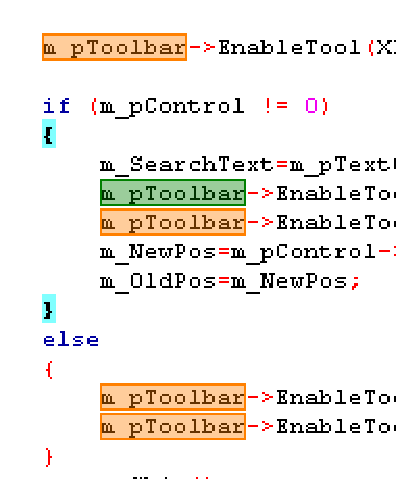
\includegraphics{incremental_search_example}

Si la chaîne de caractère recherchée ne peut pas être trouvée dans le fichier courant, afin d'indiquer que c'est ce qui se passe, le fond du masque de recherche est affiché en rouge.

\screenshot{incremental_search_settings}{Paramètres pour la Recherche Incrémentale}

\begin{description}
\item[ESC] Quitte le module de Recherche Incrémentale.
\item[ALT-Suppr] Efface l'entrée du champ de recherche incrémentale.
\end{description}

Les icônes de la barre d’outils de Recherche Incrémentale ont les significations suivantes :

\begin{description}
\item[
\includegraphics{incremental_search_clear}] Suppression du texte dans le masque de recherche de la barre d'outils de Recherche Incrémentale.
\item[
\includegraphics{incremental_search_previous},
\includegraphics{incremental_search_next}] Navigation dans les occurrences de chaîne recherchée.
\item[
\includegraphics{incremental_search_highlight}] En cliquant sur ce bouton ce sont toutes les occurrences de la chaîne recherchée qui sont surlignées en couleur, pas seulement la première.
\item[
\includegraphics{incremental_search_selected}] Activer cette option réduit le champ de recherche au passage de texte marqué dans l'éditeur.
\item[
\includegraphics{incremental_search_matchcase}] Cette option signifie que la recherche sera sensible à la casse (respect des majuscules et minuscules).
\item[
\includegraphics{incremental_search_regex}] Valider les expressions régulières dans le champ d'entrée de la recherche incrémentale.
\end{description}

\hint{Le paramétrage standard de cette barre d'outil peut être configuré dans \menu{Paramètres,Éditeur,Recherche Incrémentale}.}

%\screenshot{incremental_search_settings}{Paramètres pour la Recherche Incrémentale}
